% $Header$

\documentclass[aspectratio=1610]{beamer}

\mode<presentation>
{%
  \usetheme{Boadilla}
}


\usepackage[english]{babel}
\usepackage[utf8]{inputenc}
\usepackage[T1]{fontenc}

\usepackage{%
    animate,
    graphicx,
    varwidth,
    tcolorbox,
    clrscode3e,
    tikz,
    mathtools,
    forest,
}

\usetikzlibrary{overlay-beamer-styles,matrix}

\graphicspath{{../../imgs/hash/}}

% alert a whole line (especially for algorithms)
\newcommand{\alertline}{%
 \usebeamercolor[fg]{normal text}%
 \only{\usebeamercolor[fg]{alerted text}}}

% floor command
\newcommand{\floor}[1]{\left\lfloor #1 \right\rfloor}

\title[ALG25 - Lecture 7]
{Hash Tables}

\subtitle
{Algorithms and Datastructures, F25, Lecture 7}

\author[Andreas H. Høeg-Petersen]
{Andreas Holck Høeg-Petersen}

\institute[AAU]{%
  Department of Computer Science\\
  Aalborg University
}

\date {\today}

\pgfdeclareimage[height=0.5cm]{university-logo}{../../imgs/aau-logo}
\logo{%
    \begin{tikzpicture}[overlay,remember picture]
        \node[left=0.2cm] at (current page.30){\pgfuseimage{university-logo}};
    \end{tikzpicture}
}

\AtBeginSection[]
{%
  \begin{frame}<beamer>{Outline}
    \tableofcontents[currentsection,currentsubsection]
  \end{frame}
}


\begin{document}

\begin{frame}
  \titlepage
\end{frame}

\begin{frame}{Opdateringer}{}
    \begin{itemize}[<+->]
        \small
        \item Næste programmeringsopgave er ude --- har I alle set den?
            \begin{itemize}
                \item Der vil være lidt ekstra tid til exercises i dag, og det
                    er blandt andet, så I eventuelt kan arbejde lidt med opgaven
            \end{itemize}
    \end{itemize}
\end{frame}


\begin{frame}{Outline}
  \tableofcontents
\end{frame}

\section{Direct-Address Tables}

\begin{frame}{Symbol tables}{Associer en nøgle med en værdi}
    Et \alert{symbol table} er en data struktur, der kan mappe fra en nøgle til
    en værdi (eller \alert{sattelit data}).

    \begin{itemize}[<+(1)->]
        \item Vi har set dette med \alert{binære søgetræer}, f.eks.\ i jeres
            programmeringsopgave, hvor I associere en dato med en person
        \item Et simpelt array kan faktisk også betragtes som et symbol table
            --- men hvad er så nøglen, og hvad er værdien?
            \begin{itemize}
                \item Nøglen er indexet og værdien er elementet på det index
            \end{itemize}
        \item Symbol tables --- som også kaldes \alert{dictionaries} --- skal
            understøtte operationerne $\proc{Insert}$, $\proc{Search}$ og
            $\proc{Delete}$
        \item Hash tables er en effektiv datastruktur til dette formål, der kan
            understøtte alle operationerne i $O(1)$ tid!
    \end{itemize}
\end{frame}

\begin{frame}{Direct-Address Tables}{Basically bare et array}
    Den simpleste måde at implementere er bare med et array --- dette kaldes en
    \alert{direct-address table}.

    \begin{columns}
        \small
        \column{.5\textwidth}
        \begin{itemize}[<+(1)->]
            \item Vi har en applikation, hvor vi skal kunne opbevare elementer,
                der alle sammen har en unik nøgle associeret med dem
            \item Nøglerne stammer fra et \alert{univers} af nøgler $U =
                \{0,1,\ldots,m-1\}$
            \item Vi kan repræsentere vores tabel med et array $T[0:m-1]$, hvor
                vi har plads til $m$ elementer
            \item Elementet med nøgle $k$ finder vi så på plads $T[k]$ (hvor
                $T[k] = \const{NIL}$, hvis ikke elementet findes i $T$)
            \item Med $m$ nøgler i $U$ og $n$ elementer i $T$ er der altså $m -
                n$ tomme pladser i $T$
            \item Alle operationer er trivielle og kører i $O(1)$ tid
        \end{itemize}
    
        \column{.5\textwidth}
        \begin{figure}[h]
            \centering
            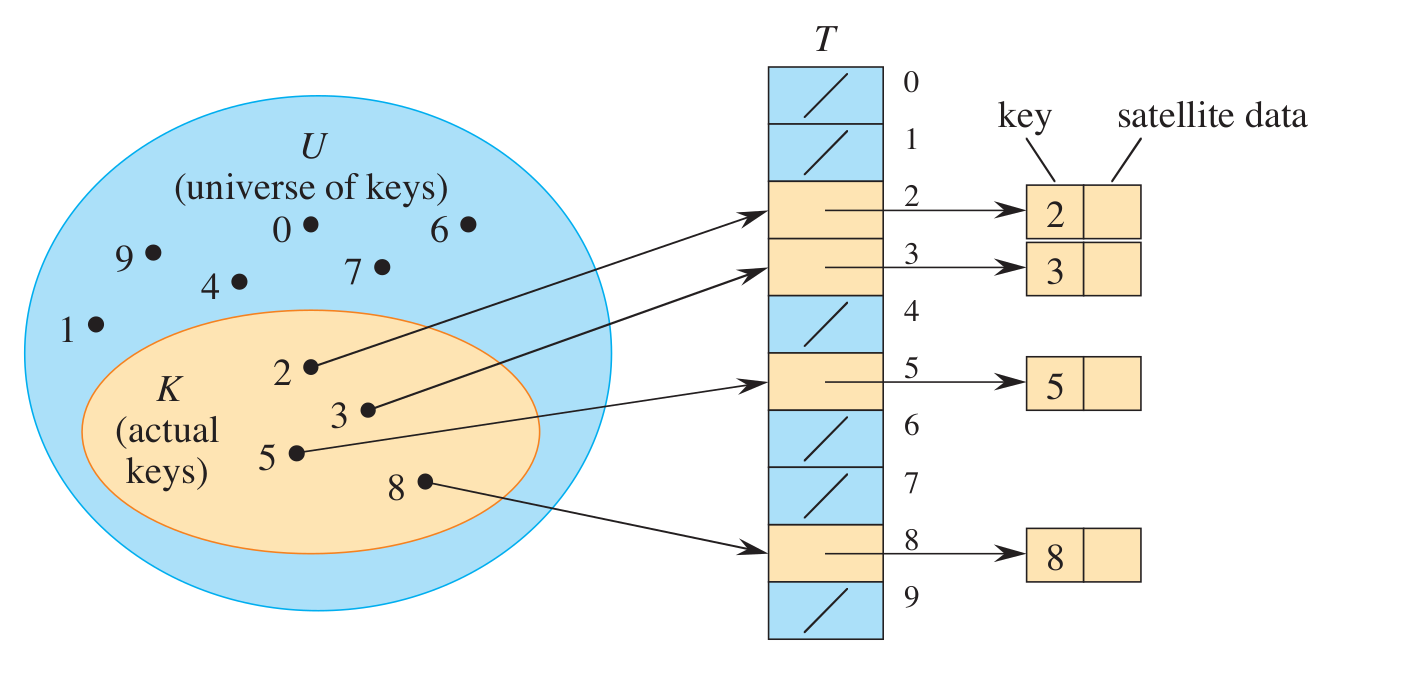
\includegraphics[width=\textwidth]{direct-address-table}
        \end{figure}
    \end{columns}
\end{frame}


\begin{frame}{Direct-Address Tables}{Eksempel}

    \begin{columns}
        \small
        \column{.5\textwidth}
        \textbf{Eksempel}
        \begin{itemize}[<+(1)->]
            \item Vi har fået en tekst og vil gerne tælle, hvor mange gange
                hvert ord optræder
            \item Vi bruger en tabel, hvor ordene er nøgler og antal forekomster
                er værdierne
            \item Vi kan associere unikke nøgler til ordene ved at bruge deres
                position, når de er sorteret i alfabetisk rækkefølge
            \item Lad os sige, at der er 500.000 danske ord, så vi kunne have
                følgende:
                \begin{itemize}
                    \item $\attrib{\text{`Abe'}}{key} = 0$ 
                    \item $\attrib{\text{`Mark'}}{key} = 250.000$
                    \item $\attrib{\text{`År'}}{key} = 499.999$ 
                \end{itemize}
        \end{itemize}
    
        \column{.5\textwidth}
        \begin{figure}[h]
            \centering
            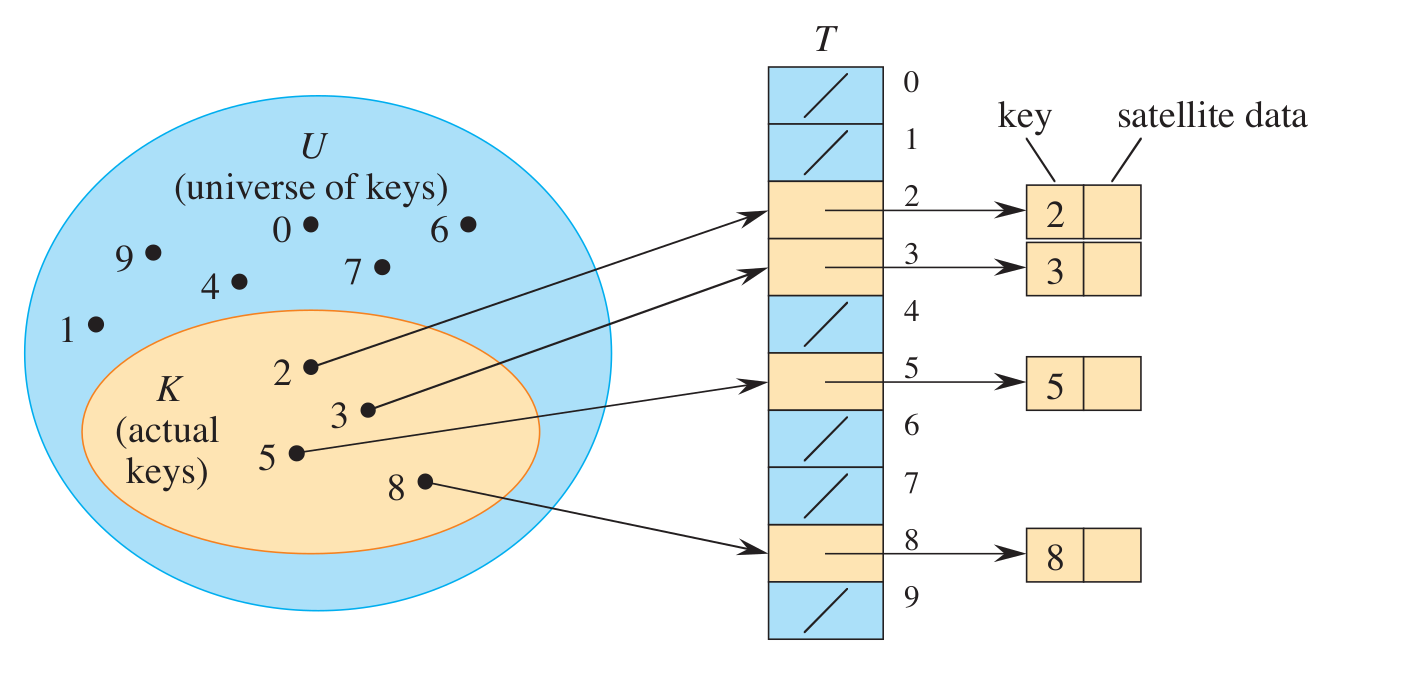
\includegraphics[width=\textwidth]{direct-address-table}
        \end{figure}
    \end{columns}
\end{frame}

\begin{frame}{Direct-Address Tables}{Eksempel}
    \begin{center}
        \textbf{PROBLEM!!!}
    \end{center}
\end{frame}


\begin{frame}{Direct-Address Tables}{Eksempel}

    \begin{columns}
        \small
        \column{.5\textwidth}
        \textbf{Eksempel}
        \begin{itemize}[<+(1)->]
            \item Vi møder måske kun 100-200 forskellige ord i artiklen, men
                vores tabel har plads til mere end 1000 gange så mange!
            \item Direct-Address tables er ikke smarte, når $U$ er langt større
                end $K$ (sættet af aktuelle nøgler)
            \item Hvad værre er: vi kan have at $U$ er så stort (eller
                uendeligt!), at det er umuligt at have en tabel med plads til
                alle nøgler
        \end{itemize}
    
        \column{.5\textwidth}
        \begin{figure}[h]
            \centering
            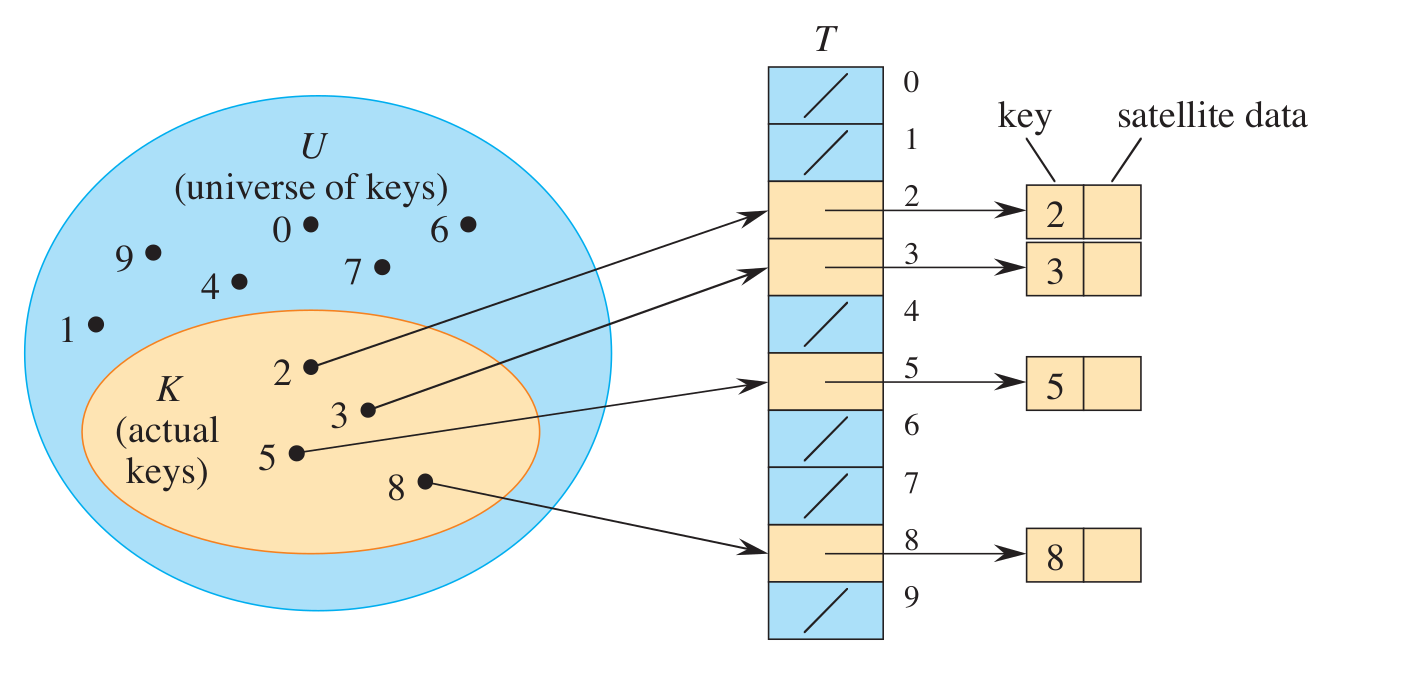
\includegraphics[width=\textwidth]{direct-address-table}
        \end{figure}
    \end{columns}
\end{frame}


\section{Hash tables}

\begin{frame}{Hashing}{Har ikke noget med weed at gøre}
    I stedet for at have plads til alle $|U|$ nøgler, kan vi bruge en
    \alert{hash funktion} til at mappe fra en nøgle til en plads i et
    \alert{hash table}.

    \begin{columns}
        \column{.5\textwidth}
        \small
        \begin{itemize}[<+(1)->]
            \item At `hashe' betyder at skære eller hugge noget i stykker
                (biksemad!)
            \item En hash funktion $h: U \rightarrow \{0,1,2,\ldots,m-1\}$ er en
                funktion fra universet af nøgler til et tal mellem 0 og $m-1$
                \begin{itemize}
                    \item Eksempel: $h(k) = k \mod m$
                \end{itemize}
            \item Vores hash table $T[0:m-1]$ er et array med plads til $m$
                elementer, og vi antager at $m \ll |U|$ (altså at $m$ er
                \alert{meget mindre} end størrelsen på $U$)
            \item Dermed står elementet med nøgle $k$ på plads $T[h(k)]$
        \end{itemize}
    
        \column{.5\textwidth}
        \begin{figure}[h]
            \centering
            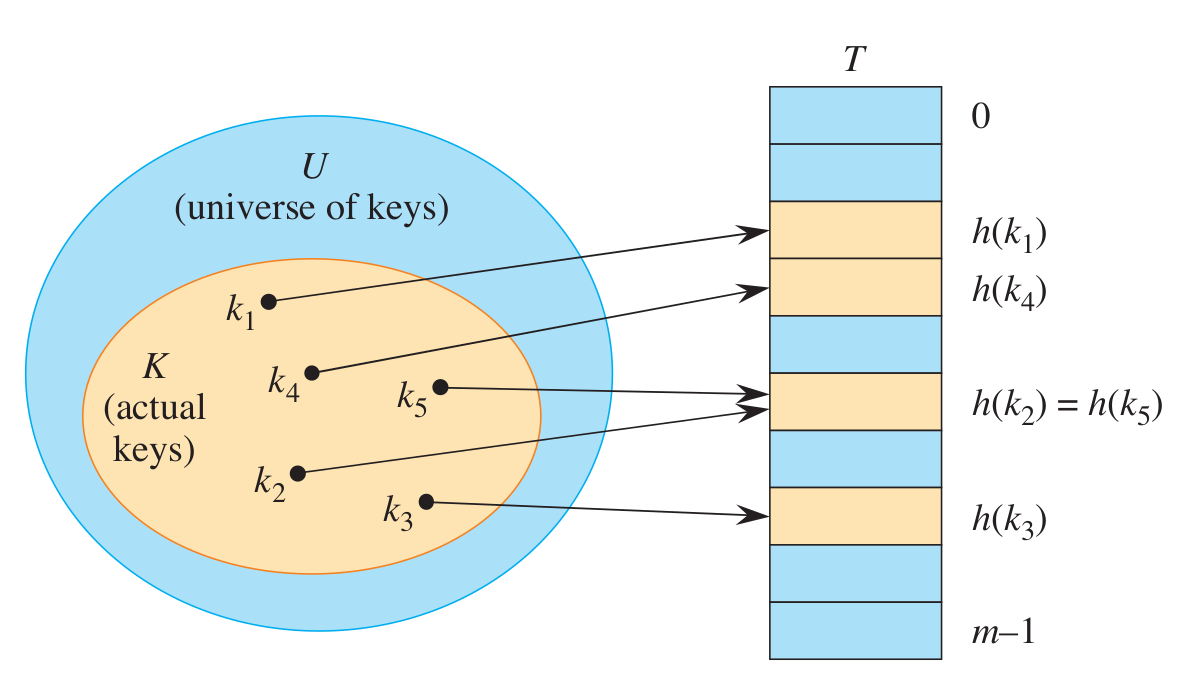
\includegraphics[width=\textwidth]{hash-table}
        \end{figure}
    \end{columns}
\end{frame}


\begin{frame}{Hashing}{}
    \begin{center}
        Problem\ldots?
    \end{center}
\end{frame}


\begin{frame}{Hashing}{Kollisioner}
    \begin{itemize}[<+->]
        \item To (eller flere) nøgler kan risikere at hash til samme værdi,
            dvs.\ $h(k_1) = h(k_2)$
        \item Dette skaber en såkaldt \alert{kollision}, da begge nøgler nu vil
            skulle stå på den samme plads i $T$
        \item Eftersom $m < |U|$, så kan kollisioner ikke undgåes
        \item Derfor skal vi dels
            \begin{enumerate}
                \item Finde en teknik for at konstruere hash-funktioner, der
                    reducerer antallet af kollisioner
                \item Finde en teknik til at håndtere kollisioner, når de
                    uundgåeligt optræder
            \end{enumerate}
    \end{itemize}
\end{frame}


\begin{frame}{Hash-funktioner}{Ideelt set}
    \begin{columns}
        \column{.5\textwidth}
        \small
        \begin{itemize}[<+->]
            \item Vi antager at alle nøgler er ikke-negative heltal - hvis ikke, kan
                vi altid lave dem om til dette (f.eks.\ tage ASCII-værdien af en
                streng)
            \item Idealet er, at $h$ er en \alert{independent uniform hash function}
                \begin{itemize}
                    \item \alert{independent} vil sige, at outputtet ikke afhænger
                        af hvad andre nøgler har hashet til
                    \item \alert{uniform} vil sige, at alle $m$ værdier i $h$'s
                        værdimængde er lige sandsynlige
                \end{itemize}
            \item For at kunne sikre dette er vi nødt til at vide noget om
                distributionen af nøgler --- og det gør vi sjældent
        \end{itemize}     
            
        \column{.5\textwidth}
        \begin{figure}[h]
            \centering
            \includegraphics<5->[width=\textwidth]{n-vokaler}
            \only<5->{\caption{Antal vokaler i ord er en dårlig hash-funktion,
            der hverken er independent eller uniform}}
        \end{figure}
    \end{columns}
    
\end{frame}


\begin{frame}{Hash-funktioner}{Metoder til at designe hash-funktioner}

    \begin{columns}[t]
        \column{.5\textwidth}
        \textbf{Static hashing}
        \begin{itemize}[<+(1)->]
            \small
            \item Bruger den samme hash-funktion hver gang
            \item Her håber vi at kunne hashe på en måde, der er uafhængig af
                mønstre i input-dataen
            \item To simple udgaver
                \begin{itemize}
                    \item \alert{Divisionsmetoden}: $h(k) = k \mod m$
                        \begin{itemize}
                            \item Hurtig og effektiv
                            \item Kan være god hvis $m$ er et primtal, der ikke
                                er tæt på en 2'er-potens
                        \end{itemize}
                    \item \alert{Multiplikationsmetoden}: $h(k) = \lfloor
                        m(kA-\lfloor kA \rfloor)\rfloor$
                        \begin{itemize}
                            \item $A$ er en konstant mellem 0 og 1
                            \item $m$ kan vælges uafhængigt af $A$, og fungerer
                                godt som en 2'er-potens
                        \end{itemize}
                \end{itemize}
            \item Dog, der er ingen garantier med static hashing
        \end{itemize}    
    
        \column{.5\textwidth}
        \pause
        \textbf{Random hashing}
        \begin{itemize}[<+->]
            \small
            \item Vi definerer en \alert{familie} $\mathcal{H}$ af
                hash-funktioner, der alle mapper $U$ til $\{0,1,\ldots,m-1\}$
            \item Når vores program starter vælger vi en tilfældig hash-funktion
                $h \in \mathcal{H}$
            \item Dette beskytter imod, at en ondsindet agent kan finde $n$
                nøgler, der alle hasher til samme værdi 
            \item En familie $\mathcal{H}$ af hash-funktioner kan defineres ved
                \begin{itemize}
                    \item \alert{Talteori} --- magi med primtal og modulo
                    \item \alert{Multiplikationsmetoden} --- en sofistikeret
                        udgave af førnævnte teknik, som garenterer at
                        sandsynligheden for kollision mellem to nøgler højst er
                        $2/m$ \looseness -1
                \end{itemize}
        \end{itemize}    
    
    \end{columns}
\end{frame}


\section{Chaining}

\begin{frame}[t]{Separate chaining}{Håndtering af kollisioner}
    Når vi uundgåeligt støder ind i kollisioner, så skal vi have metoder til at
    håndtere dette.

    \begin{itemize}[<+->]
        \item Den mest simple metode kaldes \alert{chaining}
        \item Her gemmer vi en \alert{linked list} på hver plads i $T$
        \item Kollisioner løses således bare ved at tilføje elementet til listen
    \end{itemize}

    \begin{figure}[h]
        \centering
        \includegraphics<2->[width=0.8\textwidth]{chaining}
    \end{figure}
\end{frame}

\begin{frame}{Chaining}{Operation}
    Alle operationerne for dictionaries er nemme at implementere:

    \begin{columns}
        \column{.6\textwidth}
        \begin{itemize}
            \small
            \item<2-> $\proc{Insert}(T,x)$
                \begin{itemize}
                    \item Indsæt i starten af listen på $T[h(x.key)]$
                    \item $O(1)$
                \end{itemize}
            \item<3-> $\proc{Delete}(T,x)$
                \begin{itemize}
                    \item Slet $x$ fra listen på $T[h(x.key)]$
                    \item $O(1)$ (for doubly linked lists)
                \end{itemize}
            \item<4-> $\proc{Searc}(T,k)$
                \begin{itemize}
                    \item Søg efter $k$ i listen på plads $T[h(k)]$
                    \item Lineær tid proportionelt med listens længde
                \end{itemize}
        \end{itemize}
    
        \column{.4\textwidth}
        \begin{figure}[h]
            \centering
            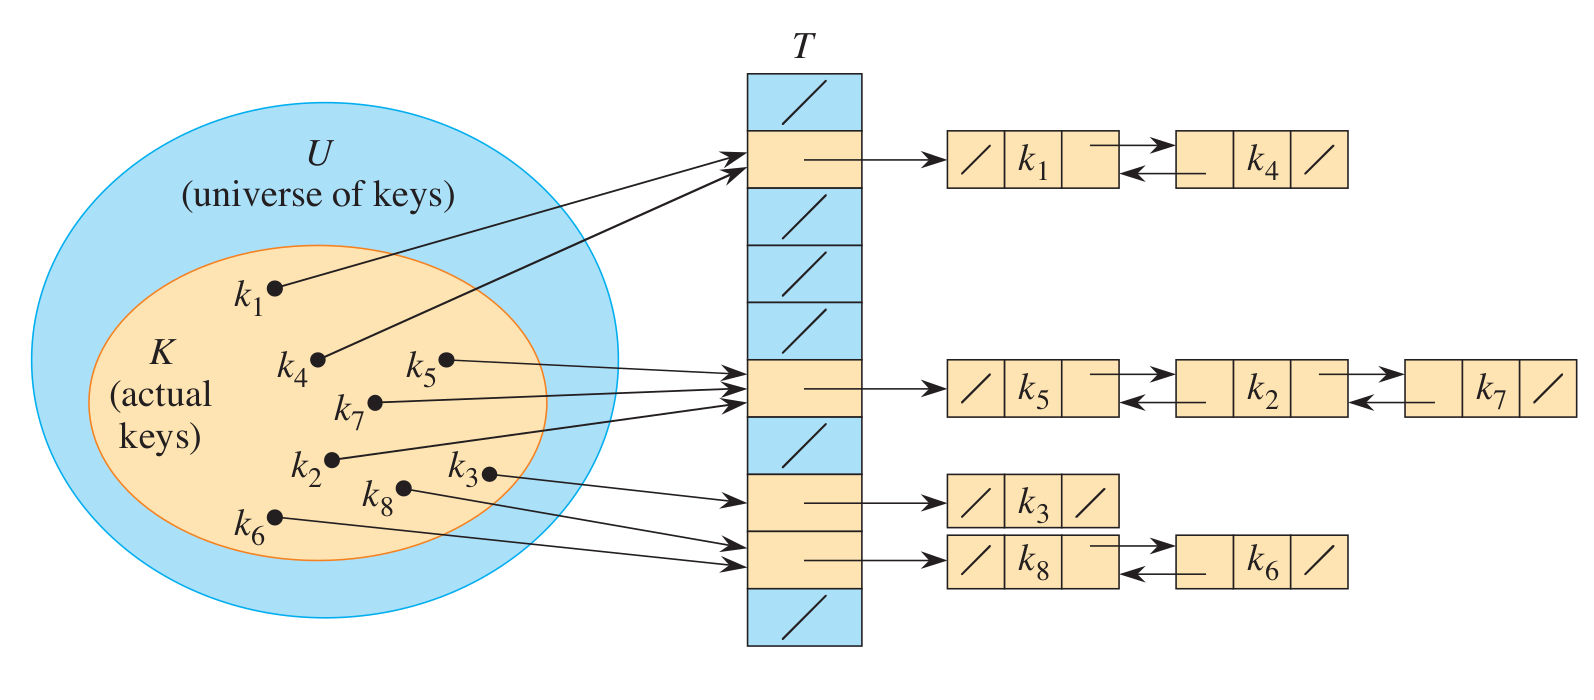
\includegraphics[width=\textwidth]{chaining}
        \end{figure}
    \end{columns}
\end{frame}


\begin{frame}{Chaining}{Kompleksitet}
    \begin{itemize}[<+->]
        \item Hvad er worst-case for $\proc{Search}$ i hash-table $T$ med $m$
            pladser og $n$ elementer (når vi bruger chaining)?
            \begin{itemize}
                \item Hvis alle nøgler hasher til samme værdi, så er det $\Theta(n)$
                \item Tydeligvis bruger vi ikke hash tables for deres worst-case
                    performance
            \end{itemize}
        \item I stedet, hvis vi antager \alert{independent uniform hashing} kan
            vi definere $\alpha = n/m$ som vores \alert{load factor} (det antal
            elementer, vi i gennemsnit forventer pr liste)
        \item Nu kan man vise (se CLRS), at søgning i en hash table med chaining
            er givet ved $\Theta(1 + \alpha)$
        \item Og hvis antallet af elementer i $T$ er proportionel med antallet
            af pladser (ie.\ $n = O(m)$), så har vi ydermere $\alpha = n/m =
            O(m)/m = O(1)$, hvilket vil sige, at også søgning er $O(1)$ i
            gennemsnit
    \end{itemize}
\end{frame}


\section{Exercises}

\begin{frame}{Exercises}{Super fedt! <3}

    På Moodle! Go! Fungerer det fint?

    \begin{figure}[h]
        \centering
        
\includegraphics[width=0.8\textwidth]{../exercises}
    \end{figure}
    
\end{frame}


\section{Open addressing}


\begin{frame}{Open addressing}{Sig farvel til pointers}
    Et populært alternativt til chaining gemmer alle elementer direkte i
    tabellen og benytter \alert{probing} til at løse kollisioner.

    \begin{itemize}[<+(1)->]
        \item Hver plads i tabellen indeholder enten et element eller
            $\const{NIL}$
        \item Da tabellen dermed kan blive fyldt, vil $n \leq m$ hvormed vores
            load factor $\alpha \leq 1$
        \item Da vi undgår pointers, frigøres der hukommelse, der i stedet kan
            bruges til at have en større tabel og dermed kortere søge-tid
        \item Men hvad er \alert{probing} så?
    \end{itemize}
\end{frame}


\begin{frame}{Open addressing}{Probing}
    \begin{columns}
        \column{.7\textwidth}
        \begin{itemize}
            \item<1-> Ideen er, at vi `prober' tabellen for en ledig plads, et index af
                gangen
            \item<2-> En \alert{probe-sekvens} er den rækkefølge, vi tjekker pladserne i
                tabellen i og er en permutation af $(0,1,\ldots,m-1)$
            \item<7-> Vi udvider hash-funktionen til at inkludere probe-nummeret som
                input:
                \begin{itemize}
                    \item $h: U \times \{0,1,\ldots,m-1\} \rightarrow
                        \{0,1,\ldots,m-1\}$
                \end{itemize}
            \item<8-> Dermed bliver probe-sekevensen en tuple $\langle
                h(k,0),h(k,1),\ldots h(k,m-1)\rangle$
        \end{itemize}
    
        \column{.3\textwidth}
        \begin{tikzpicture}[
            empty node/.style={%
                execute at begin node={},
            },
            content node/.style={%
                fill=gray!10,
                execute at begin node={####1},
            },
            ]
            \matrix (m) [
                ampersand replacement=\&,
                matrix of math nodes,
                nodes in empty cells,
                nodes={font={\ttfamily}},
                column sep=0,row sep=0,
                column 1/.style={nodes={align=center}},
                column 2/.style={%
                    nodes={%
                        text width=.5cm,
                        align=center,
                    }
                },
            ]{%
                0  \& |[content node={10}]|  \\
                1  \& |[content node={79}]|  \\
                2  \& |[empty node]|         \\
                3  \& |[empty node]|         \\
                4  \& |[content node={69}]|  \\
                5  \& |[content node={98}]|  \\
                6  \& |[empty node]|         \\
                7  \& |[content node={72}]|  \\
                8  \& |[empty node]|         \\
                9  \& |[content node={14}]|  \\
                10 \& |[empty node]|         \\
                11 \& |[content node={50}]|  \\
                12 \& |[empty node]|         \\
            };

            \draw (m-1-2.north west) rectangle (m-13-2.south east);
            \draw (m-1-2.north east) rectangle (m-13-2.south east);
            \foreach \x in {1,...,13} {%
                \draw (m-\x-2.south west) -- (m-\x-2.south east);
            };
            \draw<3->[->,rounded corners] (m-2-2.east) to [bend left] (m-6-2.east);
            \draw<4->[->,rounded corners] (m-6-2.east) to [bend left] (m-8-2.east);
            \draw<5->[->,rounded corners] (m-8-2.east) to [bend left] (m-10-2.east);
            \draw<6->[->,rounded corners] (m-10-2.east) to [bend left] (m-11-2.east);
        \end{tikzpicture}
    \end{columns}
\end{frame}


\begin{frame}{Hashing i open addressing}{}
    Hvordan hasher vi så?

    \begin{itemize}
        \item Ideelt set, så ønsker vi os \alert{independent uniform permutation
            hashing} som betyder, at probe-sekvensen har lige stor sandsynlighed
            for genere en hvilken som helst af de $m!$ permutationer af
            $(0,1,\ldots m-1)$
        \item Dette er dog meget svært at implementere (og mindre kan også gøre
            det)
        \item Vi ser på to teknikker, der generer hhv.\ $m$ og $m^2$
            probe-sekvenser:
            \begin{itemize}
                \item Lineær probing
                \item Dobbelt hashing
            \end{itemize}
    \end{itemize}
    
\end{frame}


\begin{frame}{Lineær probing}{}
    Den simpleste metode er \alert{lineær probing}:

    \[
        h(k,i) = (h'(k) + i) \mod m
    \] 

    \begin{itemize}
        \item Vi bruger en `auxiliary' hash funktion $h': U \rightarrow
            \{0,1,\ldots, m-1\}$
        \item Probe-nummeret $i$ bruges til at springe 1 plads frem hver gang
        \item Hvis $m=8$ og $h'(k) = \lfloor k/3 \rfloor$ ville vi for $k=10$ få
            probesekvensen $(3, 4, \ldots, 7, 0, 1, 2)$
        \item Nem at implementere, men kan kun generere $m$ probe-sekvenser
        \item Har en tendens til at skabe \alert{primary clustering}, ie.\ lange
            sekvenser hvor pladser er optaget
    \end{itemize}
\end{frame}

\begin{frame}{Dobbelt hashing}{}
    Faktisk er lineær probing et særtilfælde af en mere generel metode kaldet
    \alert{dobbelt hashing}:

    \begin{columns}[t]
        \column{.7\textwidth}
        \[
            h(k,i) = (h_1(k) + i h_2(k)) \mod m
        \] 

        \begin{itemize}
            \small
            \item Nu bruger vi 2 auxiliary hash funktioner, nemlig $h_1$ og $h_2$
            \item Vores første check (når $i=0$) går til plads $T[h_1(k) \mod m]$ og
                derefter springer vi $h_2(k)$ pladser frem hver gang
            \item $h_2$ kan dermed ses som en slags `step'-funktion
            \item For at garantere, at hele tabellen bliver undersøgt, så skal
                værdien af $h_2$ være et primtal relativt til $m$
                \begin{itemize}
                    \item Enten, lad $m$ være en 2'er-potens og sørg for $h_2$ altid
                        returnerer et ulige tal\ldots
                    \item \ldots\ eller lad $m$ være et primtal og sørg for at $h_2$
                        altid returnerer et tal mindre end $m$
                \end{itemize}
            \item Dette giver $m^2$ forskellige probe-sekvenser, hvilket er tæt nok
                på idealet
        \end{itemize}
    
        \column{.3\textwidth}
        \begin{figure}
            \begin{tikzpicture}[
                every node/.style={scale=0.75},
                empty node/.style={%
                    execute at begin node={},
                },
                content node/.style={%
                    fill=gray!10,
                    execute at begin node={####1},
                },
                ]
                \matrix (m) [
                ampersand replacement=\&,
                matrix of math nodes,
                nodes in empty cells,
                nodes={font={\ttfamily}},
                column sep=0,row sep=0,
                column 1/.style={nodes={align=center}},
                column 2/.style={%
                    nodes={%
                        text width=.5cm,
                        align=center,
                    }
                },
                ]{%
                    0  \& |[content node={26}]|  \\
                    1  \& |[content node={79}]|  \\
                    2  \& |[empty node]|         \\
                    3  \& |[empty node]|         \\
                    4  \& |[content node={69}]|  \\
                    5  \& |[content node={98}]|  \\
                    6  \& |[empty node]|         \\
                    7  \& |[content node={72}]|  \\
                    8  \& |[empty node]|         \\
                    9  \& |[content node={14}]|  \\
                    10 \& |[empty node]|         \\
                    11 \& |[content node={50}]|  \\
                    12 \& |[empty node]|         \\
                };

                \draw (m-1-2.north west) rectangle (m-13-2.south east);
                \draw (m-1-2.north east) rectangle (m-13-2.south east);
                \foreach \x in {1,...,13} {%
                    \draw (m-\x-2.south west) -- (m-\x-2.south east);
                };
            \draw[->,rounded corners] (m-2-2.east) to [bend left] (m-6-2.east);
            \draw[->,rounded corners] (m-6-2.east) to [bend left] (m-10-2.east);
        \end{tikzpicture}
        \caption{%
            \footnotesize Eksempel på dobbelt hashing hvor $h_1(k) = k \mod 13$
            og $h_2(k) = 1 + (k \mod 11)$
        }
        \end{figure}
    \end{columns}
\end{frame}


\begin{frame}{Insertion}{Finally, some pseudo-kode!}
    Vi slutter med at se på koden for $\proc{Insert}$, $\proc{Search}$ og\ldots
    $\proc{Delete}$?

    \begin{columns}
        \column{.4\textwidth}
        \begin{block}{$\proc{Hash-Insert}(T,k)$}
        
            \vspace{-\abovedisplayskip}
            \begin{codebox}
                \li \alertline<2>$i \gets 0$
                \li \Repeat
                \li     \alertline<3>$q \gets h(k,i)$
                \li     \alertline<4>\If $T[q] \isequal \const{NIL}$
                        \Then
                \li         \alertline<4>$T[q] \gets k$
                \li         \alertline<4>\Return $q$
                \li     \alertline<5>\Else $i \gets i + 1$
                        \End
                \li \Until $i \isequal m$
                \li \alertline<6>\Error `hash table overflow'
            \end{codebox}
        \end{block}
    
        \column{.6\textwidth}
        \begin{itemize}
            \item<2-> Vi starter med at initialisere proben til 0
            \item<3-> Så hasher vi nøglen og probe-nummeret og gemmer værdien i $q$
            \item<4-> Hvis $T[q]$ er tom, så indsætter vi $k$ og returnerer $q$
            \item<5-> Ellers inkrementerer vi $i$ og gentager indtil $i = m$
            \item<6-> Når vi ud af loopet, så er vores tabel helt fyldt
        \end{itemize}
    \end{columns}
\end{frame}

\begin{frame}{Search}{Same same but different}
    Søgning er næsten identisk:

    \begin{columns}
        \column{.4\textwidth}
        \begin{block}{$\proc{Hash-Search}(T,k)$}
        
            \vspace{-\abovedisplayskip}
            \begin{codebox}
                \li \alertline<2>$i \gets 0$
                \li \alertline<6>\Repeat
                \li     \alertline<3>$q \gets h(k,i)$
                \li     \alertline<4>\If $T[q] \isequal \const{NIL}$
                        \Then
                \li         \alertline<4>\Return $q$
                \li     \alertline<5>\Else $i \gets i + 1$
                        \End
                \li \alertline<6>\Until $T[q] \isequal \const{NIL}$ or $i \isequal m$
                \li \alertline<7>\Error `hash table overflow'
            \end{codebox}
        \end{block}
    
        \column{.6\textwidth}
        \begin{itemize}
            \item<2-> Vi starter med at initialisere proben til 0
            \item<3-> Så hasher vi nøglen og probe-nummeret og gemmer værdien i $q$
            \item<4-> Hvis $T[q]$ er tom, så returnerer vi $q$
            \item<5-> Ellers inkrementerer vi $i$\ldots
            \item<6->\ldots\ og gentager indtil vi finder en tom plads eller
                $i=m$
            \item<7-> Når vi ud af loopet, så findes $k$ ikke i $T$
        \end{itemize}
    \end{columns}
\end{frame}

\begin{frame}{Deletion}{Det må også være nemt!}
    Hvad så med deletion?
    \begin{columns}
        \column{.7\textwidth}
        \begin{itemize}
            \item<2-> Intuitivt: hvis vi vil slette et element, så indsætter vi bare
                $\const{NIL}$ på dets plads
            \item<3-> Giver det nogen problemer?
            \item<4-> Eksempel:
                \begin{itemize}
                    \item<5-> Vi sletter nøglen `98'
                    \item<6-> Nu skal vi søge efter `14', og vi tjekker først plads
                        1
                    \item<7-> Der står hverken $\const{NIL}$ eller `14', så vi
                        fortsætter
                    \item<8-> Nu tjekker vi plads 5, og der står $\const{NIL}$,
                        fordi vi har slettet `98'
                    \item<9-> Dermed returnerer vi $\const{NIL}$, selvom `14'
                        faktisk findes længere nede i tabellen!
                \end{itemize}
        \end{itemize}

        \column{.3\textwidth}
        \begin{center}
            \begin{tikzpicture}[
                every node/.style={scale=0.75},
                empty node/.style={%
                    execute at begin node={},
                },
                content node/.style={%
                    fill=gray!10,
                    execute at begin node={####1},
                },
                ]
                \matrix (m) [
                ampersand replacement=\&,
                visible on=<4->,
                matrix of math nodes,
                nodes in empty cells,
                nodes={font={\ttfamily}},
                column sep=0,row sep=0,
                column 1/.style={nodes={align=center}},
                column 2/.style={%
                    nodes={%
                        text width=.5cm,
                        align=center,
                    }
                },
                ]{%
                    0  \& |[content node={26}]|  \\
                    1  \& |[content node={79}]|  \\
                    2  \& |[empty node]|         \\
                    3  \& |[empty node]|         \\
                    4  \& |[content node={69}]|  \\
                    5  \& |[fill=gray!10, visible on=<-5>]| 98  \\
                    6  \& |[empty node]|         \\
                    7  \& |[content node={72}]|  \\
                    8  \& |[empty node]|         \\
                    9  \& |[content node={14}]|  \\
                    10 \& |[empty node]|         \\
                    11 \& |[content node={50}]|  \\
                    12 \& |[empty node]|         \\
                };

                \draw (m-1-2.north west) rectangle (m-13-2.south east);
                \draw (m-1-2.north east) rectangle (m-13-2.south east);
                \foreach \x in {1,...,13} {%
                    \draw (m-\x-2.south west) -- (m-\x-2.south east);
                };
            \draw<6->[->] ([xshift=3mm]m-2-2.east) -- (m-2-2.east);
            \draw<8->[->] (m-2-2.east) to [bend left] (m-6-2.east);
        \end{tikzpicture}
    \end{center}
    \end{columns}
\end{frame}


\begin{frame}{Deletion}{Hva' gør vi så?}
    Det korte svar er, lad være at bruge open addressing, hvis deletion er
    nødvendigt.

    \begin{itemize}
        \item Vi kan ikke bare markere en plads med $\const{NIL}$
        \item En løsning er at bruge en anden speciel værdi $\const{DELETED}$
        \item Så skal vi bare modificere $\proc{Hash-Insert}$ til at behandle
            sådanne elementer som $\const{NIL}$
        \item Anses som problematisk grundet dårlig performance ved mange
            deletions
        \item \alert{Take-home message:} Hvis man vil understøtte deletion er
            det bedre at bruge chaining
    \end{itemize}
\end{frame}

\begin{frame}{Tak for i dag!}{Flere exercises..}

    Den bedste måde ikke at snyde sig selv på er lave exercises!

    \begin{figure}[h]
        \centering
        
\includegraphics[width=0.8\textwidth]{../exercises}
    \end{figure}
    
\end{frame}



\end{document}


